% no notes
\documentclass{beamer}
% notes and slides
%\documentclass[notes]{beamer}
% notes only
% \documentclass[notes=only]{beamer}
\usepackage{graphicx} % Allows including images
\usepackage{booktabs} % Allows the use of \toprule, \midrule and \bottomrule in tables
\usepackage{multirow}
\usepackage{multimedia}
\usepackage{tikz}
\usepackage{circuitikz}
\usepackage{url}
\usepackage{pgfplots}
\pgfplotsset{compat=newest}
\usepgfplotslibrary{groupplots,dateplot}
\usetikzlibrary{patterns,shapes.arrows}
\usepackage{standalone}
\usepackage{adjustbox}
\usepackage{lmodern}
\usepackage{pgfplots}
\usepackage{amsmath}
\usepackage{amsthm}
\usepackage{multimedia}
\usepackage{standalone}
\usepackage{csquotes}


\PassOptionsToPackage{american}{babel} % change this to your language(s), main language last
% Spanish languages need extra options in order to work with this template
% \PassOptionsToPackage{spanish,es-lcroman}{babel}
\usepackage{babel}

\PassOptionsToPackage{%
  backend=biber,bibencoding=utf8, %instead of bibtex
  %backend=bibtex8,bibencoding=ascii,%
  language=auto,%
  style=numeric-comp,%
  %style=authoryear-comp, % Author 1999, 2010
  %bibstyle=authoryear,dashed=false, % dashed: substitute rep. author with ---
  style=alphabetic,
  sorting=nyt, % name, year, title
  maxbibnames=10, % default: 3, et al.
  %backref=true,%
  %natbib=true % natbib compatibility mode (\citep and \citet still work)
}{biblatex}
\usepackage{biblatex}

\addbibresource{bib.bib}

\usetheme{metropolis}           % Use metropolis theme
\setbeamertemplate{caption}[default]
\title{Welcome to the Machine Learning for Principal Investigators Course}
\date{\today}
\institute{High-Performance Computing and Analytics Lab, Universität Bonn}
\author{Moritz Wolter}

\titlegraphic{
\includegraphics[width=2.00cm]{UNI_Bonn_Logo_Standard_RZ.pdf}}
\begin{document}
    \maketitle

    \begin{frame}
    \frametitle{Overview} 
    \tableofcontents
    \end{frame}

    \section{Organization}
    \begin{frame}{Who are we?}
      Instructors
      \begin{itemize}
        \item Elena Trunz, Postdoc with the Visual Computing Group
        \begin{itemize}
          \item trunz@cs.uni-bonn.de
        \end{itemize}
        \item Lokesh Veeramacheneni, PhD student with the HPCA Lab
        \begin{itemize}
          \item lokiv@uni-bonn.de
        \end{itemize}
        \item Moritz Wolter, Postdoc with the HPCA Lab
        \begin{itemize}
          \item moritz.wolter@uni-bonn.de
        \end{itemize}
      \end{itemize}
      Teaching Assistants:
      \begin{itemize}
        \item Niklas Kerkfeld, Master student Computer Science
        \item Zahra Ganji, Master student Computer Science
      \end{itemize}
    \end{frame}

    \begin{frame}{Course Material}
      \begin{itemize}
        \item  We will upload GitHub-Classroom links, 
               Lecture recordings and slides onto Ecampus.
        \begin{itemize}
          \item \url{https://ecampus.uni-bonn.de/}
          \item To access eCampus, you need a UniID $\rightarrow$ helpdesk HRZ.
        \end{itemize}
        \item You can opt out of GitHub use. We provide zip files via Ecampus.
        \item We envision a hands-on course experience.
        \item You should be able to gain an intuition
              for modern machine learning algorithms and possible applications.
        \item Many exercises come with unit tests, which allow you to check your work.
      \end{itemize}
    \end{frame}

    \begin{frame}{Github Classroom}
      \begin{itemize}
        \item We will archive the GitHub Classroom in approximately one year.
        \item After the course, download the material or create a fork in your account for long-term access.
        \item Your repositories will appear at \url{https://github.com/Machine-Learning-for-PIs}.
        \item You can opt out of GitHub use. We also provide zip files via Ecampus.
      \end{itemize}
       

    \end{frame}

    \begin{frame}{Course Philosophy}
      \begin{itemize}
        \item Understand key methods 
        \item and use these.
        \item Understand resource needs.
        \item Learn how to supervise with software engineering and best practices in mind. 
      \end{itemize}
    \end{frame}

    \section{Machine Learning Applications}
    \begin{frame}{Machine learning is everywhere}
        \begin{itemize}
          \item Image processing
          \item Protein structure prediction
          \item Language processing
          \item Virtual personal assistants
          \item Fraud detection
          \item Autonomous robots
          \item Recommendation systems
          \item Photo editing
          \item $\dots$
        \end{itemize}
    \end{frame}
  
    \begin{frame}{Example: Medical image processing \cite{esann2024wolter}}
      \begin{figure}
        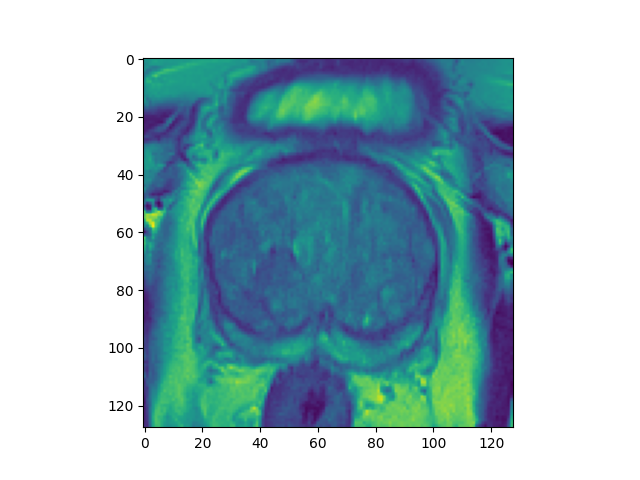
\includegraphics[width=0.32\textwidth]{./figures/prostatext2.png}
        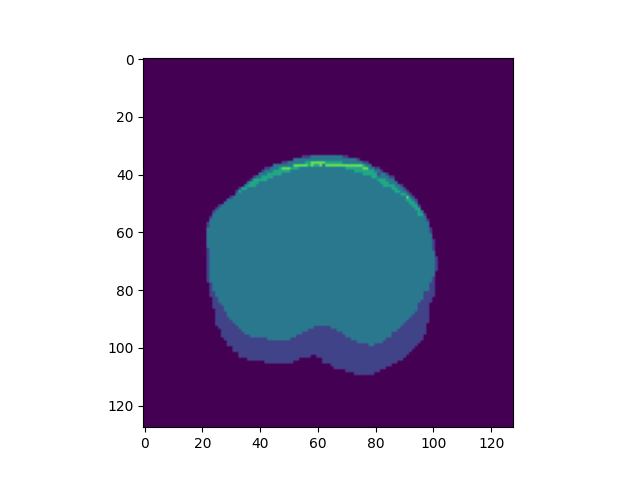
\includegraphics[width=0.32\textwidth]{./figures/prostatext2_true.png}
        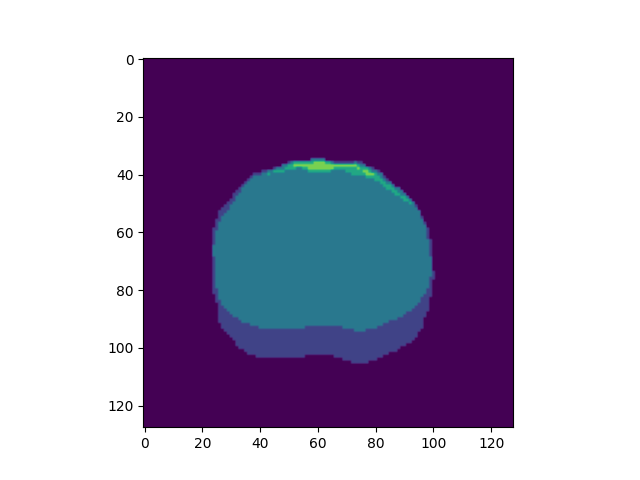
\includegraphics[width=0.32\textwidth]{./figures/prostatext2_net.png}
      \caption{A prostate (left) with expert (center) and network (right) annotation.}
      \end{figure}

      We thank Barbara Wichtmann for bringing this problem to our attention.
    \end{frame}

    \begin{frame}{Example: Processing of historical newspapers \cite{schultze2024chronicling}}
      \begin{figure}
        \includegraphics[scale=0.07]{./figures/koelnische_zeitung_9431494.jpg}
        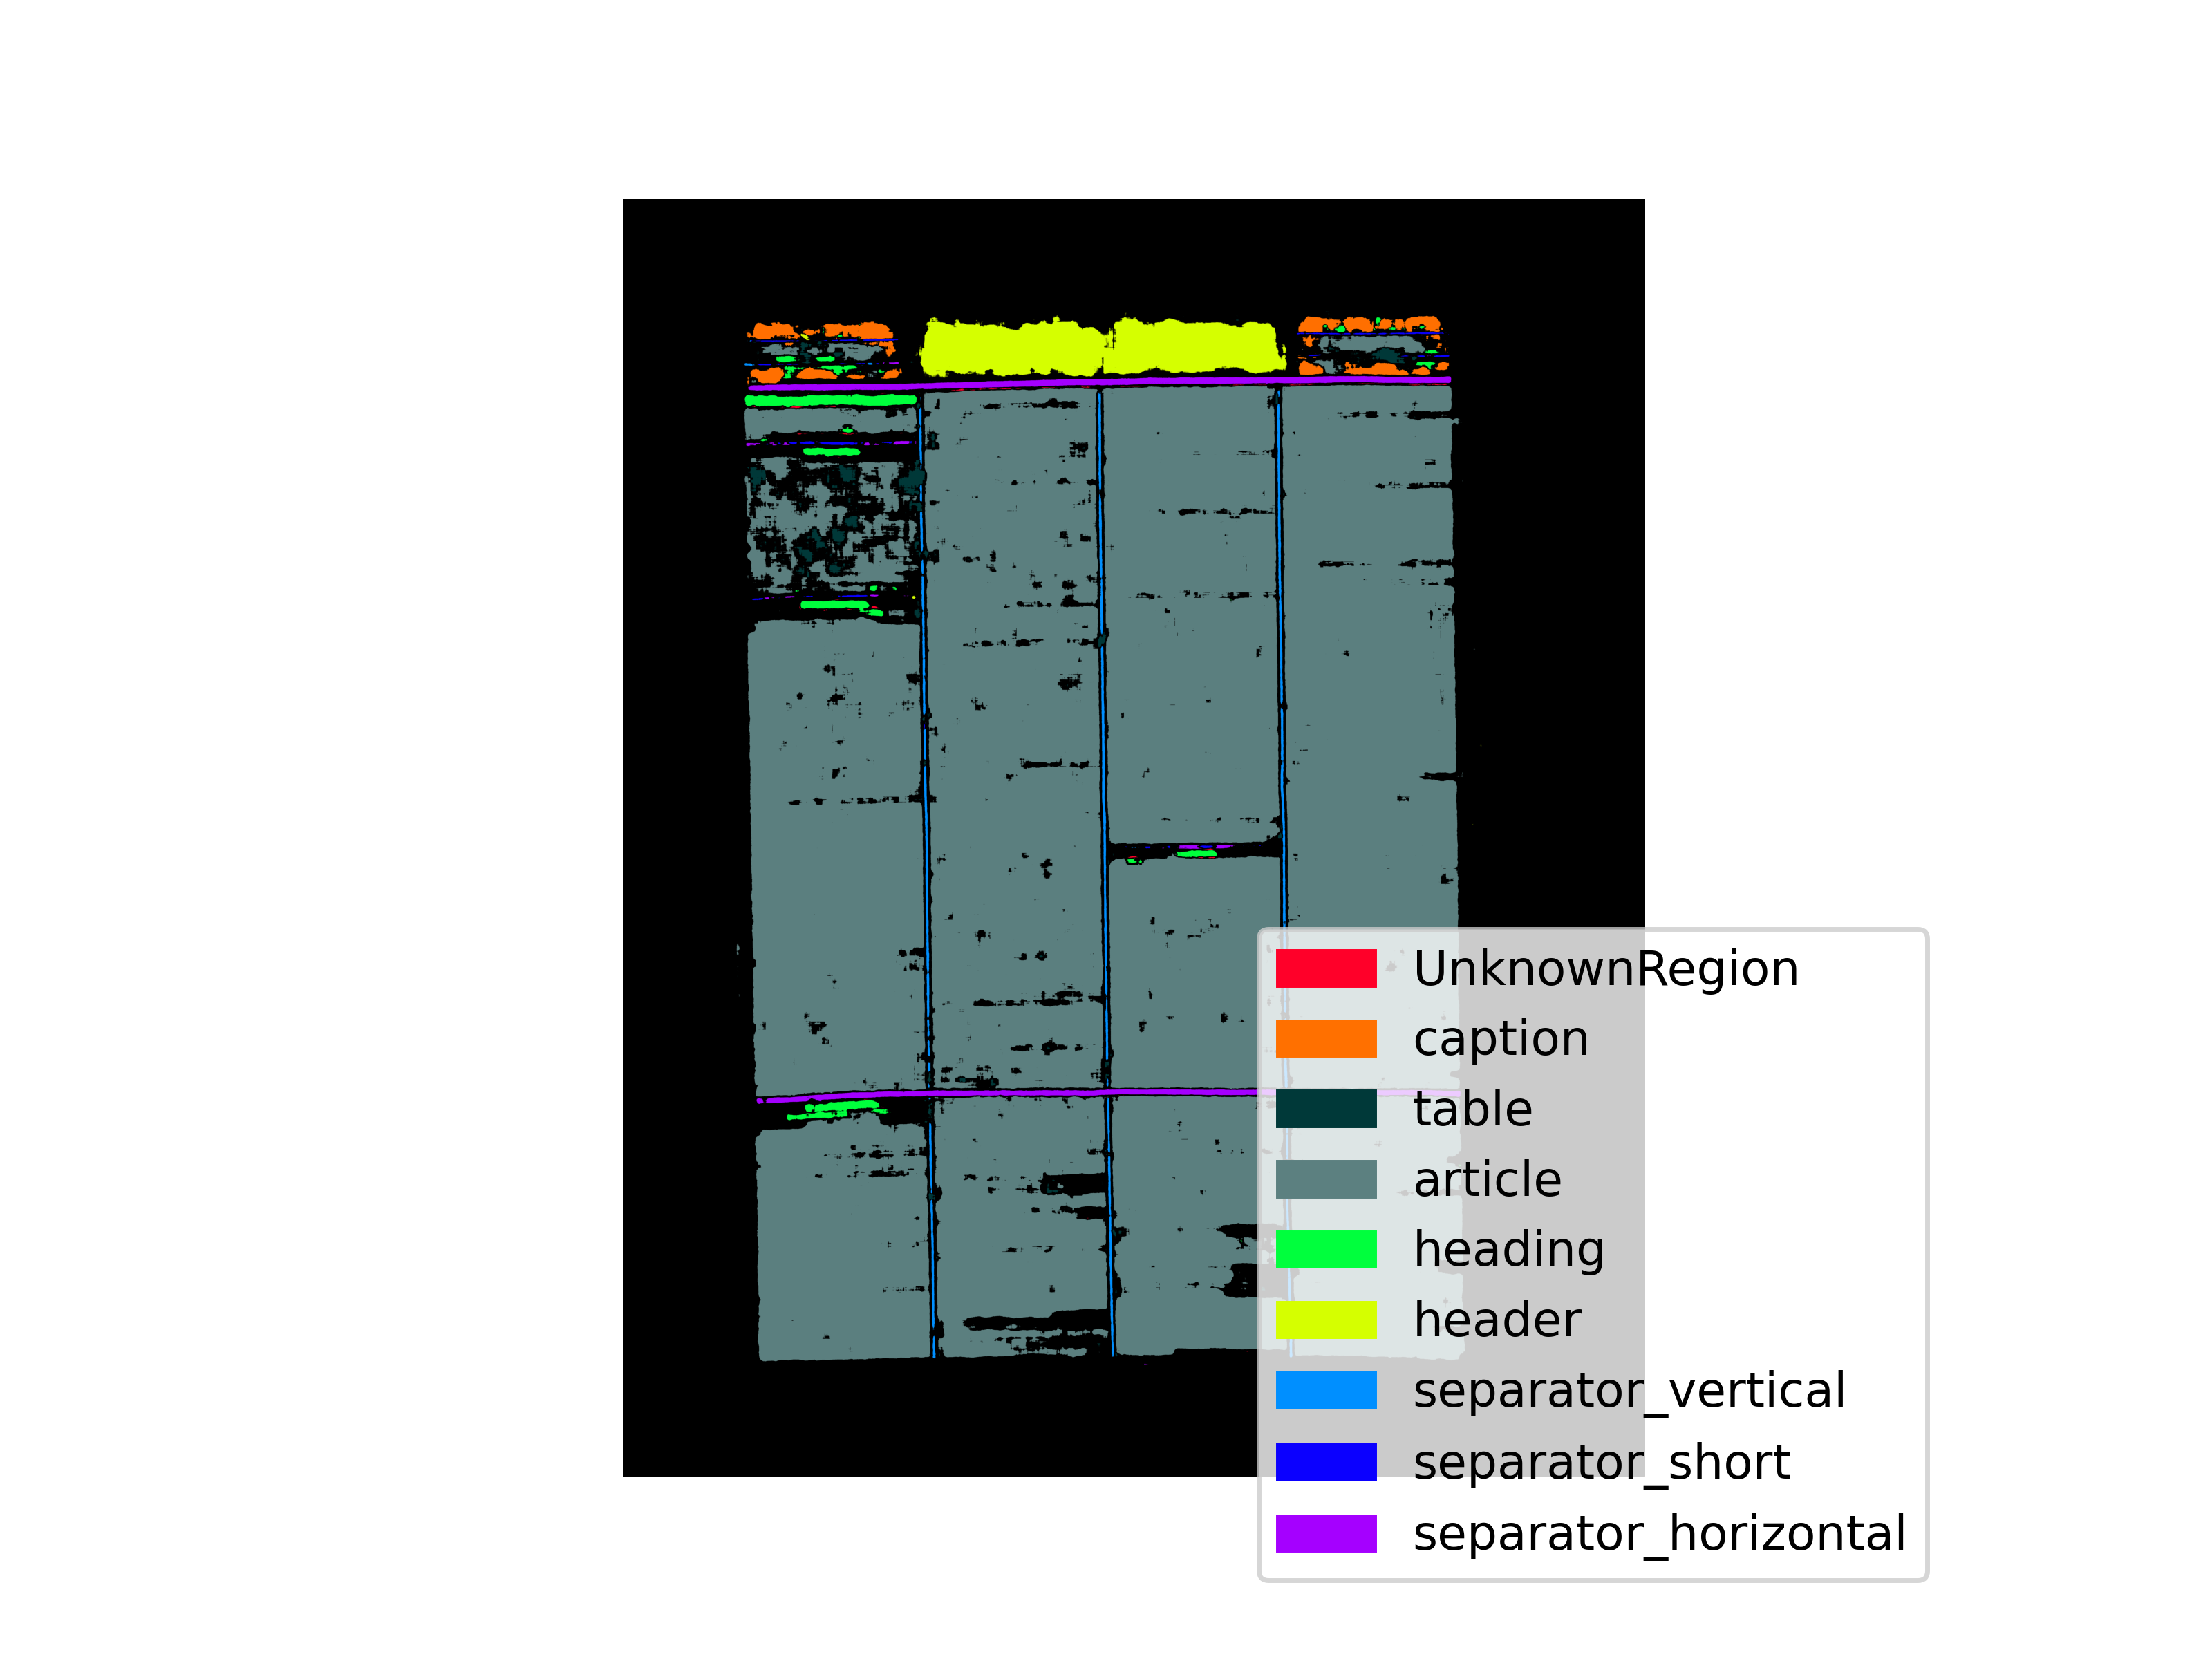
\includegraphics[scale=0.36]{./figures/segmentation_9431494.png}
      \caption{An old newspaper page and its network segmentation.}
      \end{figure}
      We thank Felix Selgert for bringing this problem to our attention.
    \end{frame}

    \begin{frame}{Stilization \cite{gatys2016image}}
      \begin{figure}
      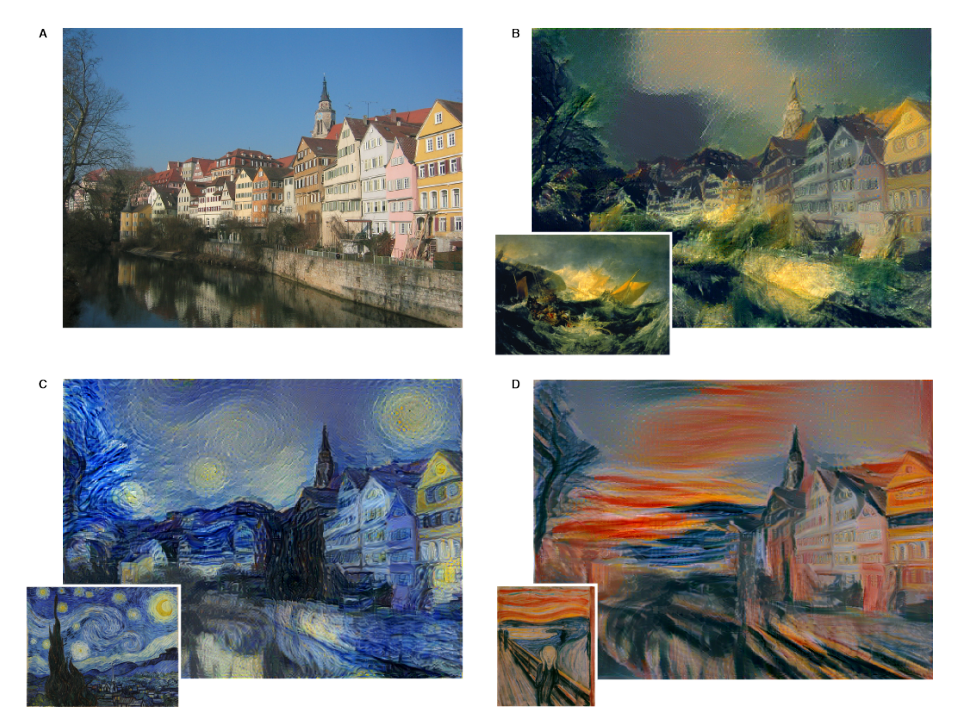
\includegraphics[width=0.6\linewidth]{./figures/neuralstyle.png}
      \end{figure}
    \end{frame}

    \begin{frame}{Image Classification \cite{DBLP:conf/nips/KrizhevskySH12}}
      \begin{figure}
        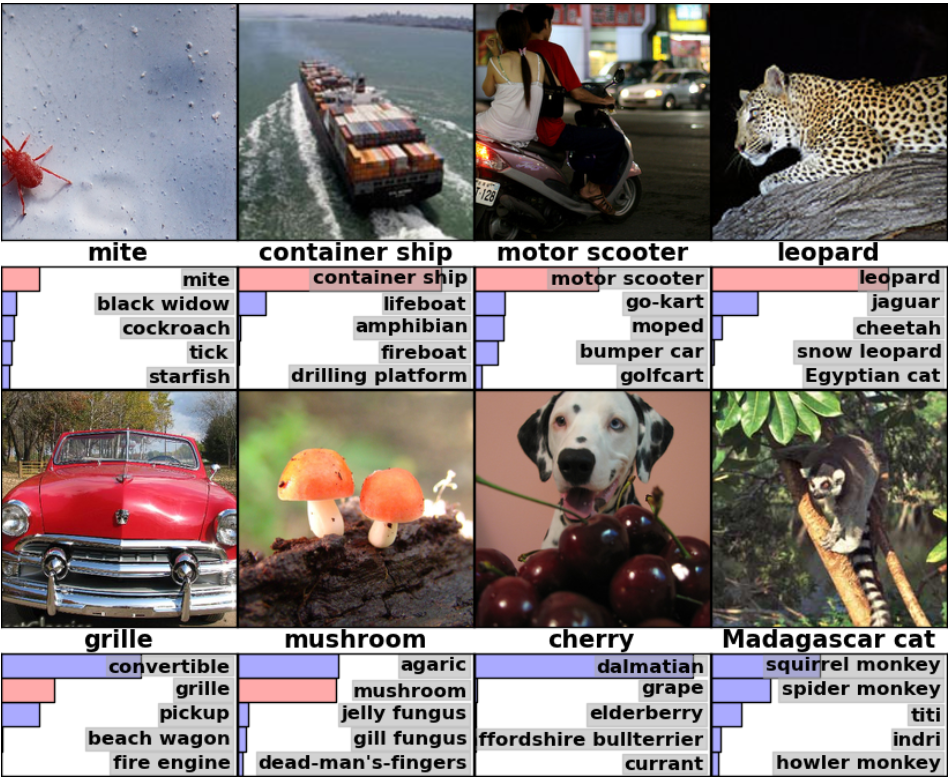
\includegraphics[scale=0.25]{./figures/classification.png}
      \end{figure}
    \end{frame}

    \begin{frame}{Image Captioning \cite{liu2023visual}}
      \begin{figure}
        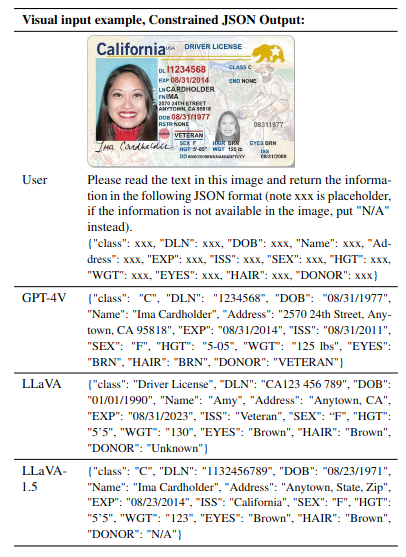
\includegraphics[scale=0.4]{./figures/visual_chat.png}
      \end{figure}
    \end{frame}

    \begin{frame}{Media Synthesis \cite{ho2020denoising}}
      \begin{figure}
        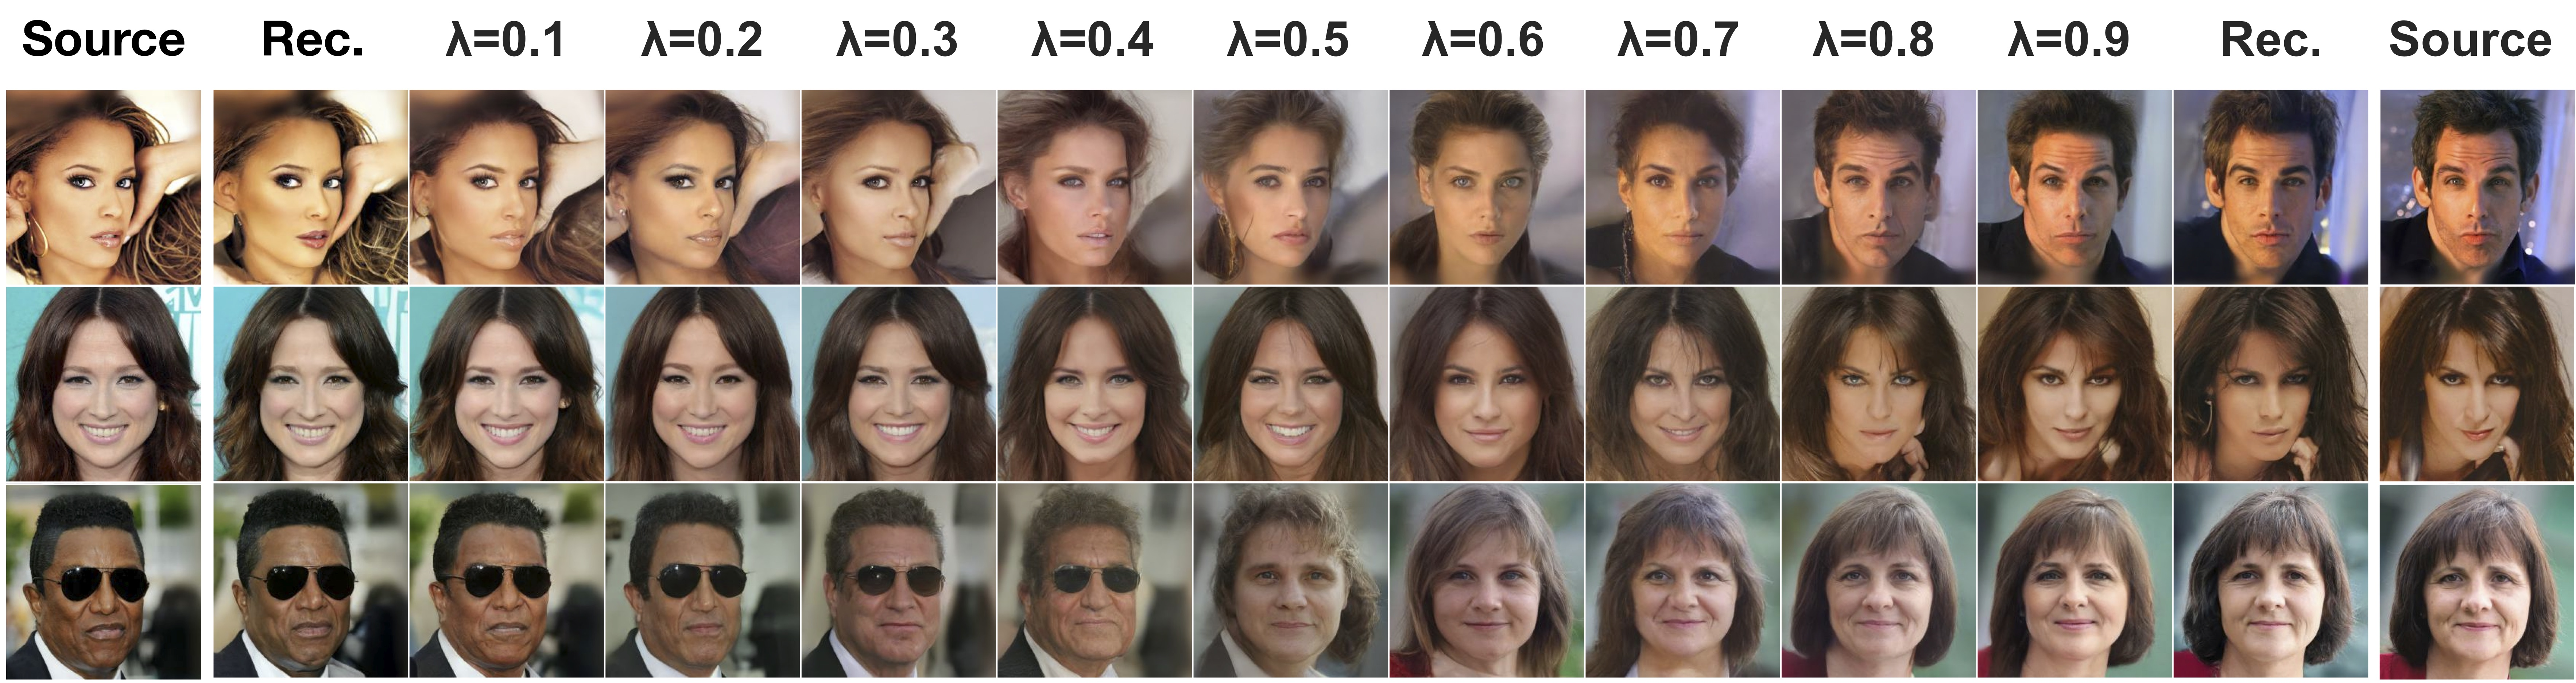
\includegraphics[width=\linewidth]{./figures/interp.jpg}
      \end{figure}
    \end{frame}


    \section{Course Contents}



    \begin{frame}{Course Outline}
      \begin{itemize}
        \item Day 1: Mathematical and software engineering foundations, based on \cite{deisenroth_faisal_ong_2020}
         \begin{itemize}
            \item  Software engineering for supervisors
            \item  Introduction, Optimization
            \item  Linear Algebra, Statistics
         \end{itemize}
        \item Foundations of machine learning, based on \cite{deisenroth_faisal_ong_2020}
        \begin{itemize}
          \item Classic Methods
          \item Support Vector Machines and Principal Component Analysis
        \end{itemize}
        \item Deep learning, based on \cite{Goodfellow_et_al_2016}
        \begin{itemize}
          \item Convolutional neural networks (CNN) for image classification
          \item CNN for image segmentation
        \end{itemize}
      \end{itemize}
    \end{frame}

    \begin{frame}{BNTrainee}
      Bonn transdisziplinäre Ausbildung in künstlicher Intelligenz \\
      Bonn transdisciplinary training in artificial intelligence
      \begin{itemize}
        \item We offer interdisciplinary machine learning projects.
        \item With CS-department: project groups/ labs, Bachelor or Master Thesis projects.
      \end{itemize}
      Website: https://trainee.informatik.uni-bonn.de/
      
      Contact:
      \begin{itemize}
        \item Elena Trunz: trunz@cs.uni-bonn.de
        \item Moritz Wolter: moritz.wolter@uni-bonn.de
      \end{itemize}
      We offer new projects at the start of each semester.
      \end{frame}
  

    \begin{frame}[allowframebreaks]{Literature}
      \printbibliography
    \end{frame}




\end{document}
